\PassOptionsToPackage{unicode=true}{hyperref} % options for packages loaded elsewhere
\PassOptionsToPackage{hyphens}{url}
%
\documentclass[12pt,a4paper,UTF8,twoside]{book}

\usepackage{lmodern}
\usepackage{setspace}
\setstretch{1.25}
\usepackage{amssymb,amsmath}
\usepackage{ifxetex,ifluatex}
\usepackage{fixltx2e} % provides \textsubscript
\ifnum 0\ifxetex 1\fi\ifluatex 1\fi=0 % if pdftex
  \usepackage[T1]{fontenc}
  \usepackage[utf8]{inputenc}
\else % if luatex or xelatex
  \ifxetex
    \usepackage{xltxtra,xunicode}
  \else
    \usepackage{fontspec}
  \fi
  \defaultfontfeatures{Mapping=tex-text,Scale=MatchLowercase}
  \newcommand{\euro}{€}

    \setmainfont[]{Times New Roman}
    \setsansfont[]{Arial}
    \setmonofont[Mapping=tex-ansi]{Inconsolata}
\fi

% use upquote if available, for straight quotes in verbatim environments
\IfFileExists{upquote.sty}{\usepackage{upquote}}{}
% use microtype if available
\IfFileExists{microtype.sty}{%
\usepackage[]{microtype}
\UseMicrotypeSet[protrusion]{basicmath} % disable protrusion for tt fonts
}{}
\usepackage{hyperref}
\hypersetup{
            pdftitle={深度学习文档集},
            pdfauthor={贝塔},
            pdfproducer={Pandoc, R Markdown, TinyTeX, knitr, bookdown, Stan},
            pdfborder={0 0 0},
            breaklinks=true}
\urlstyle{same}  % don't use monospace font for urls
\usepackage[margin=1.18in]{geometry}
\usepackage{longtable,booktabs}
% Fix footnotes in tables (requires footnote package)
\IfFileExists{footnote.sty}{\usepackage{footnote}\makesavenoteenv{longtable}}{}
\usepackage{graphicx}
\makeatletter
\def\maxwidth{\ifdim\Gin@nat@width>\linewidth\linewidth\else\Gin@nat@width\fi}
\def\maxheight{\ifdim\Gin@nat@height>\textheight\textheight\else\Gin@nat@height\fi}
\makeatother
% Scale images if necessary, so that they will not overflow the page
% margins by default, and it is still possible to overwrite the defaults
% using explicit options in \includegraphics[width, height, ...]{}
\setkeys{Gin}{width=\maxwidth,height=\maxheight,keepaspectratio}
\setlength{\emergencystretch}{3em}  % prevent overfull lines
\providecommand{\tightlist}{%
  \setlength{\itemsep}{0pt}\setlength{\parskip}{0pt}}
\setcounter{secnumdepth}{5}
% Redefines (sub)paragraphs to behave more like sections
\ifx\paragraph\undefined\else
\let\oldparagraph\paragraph
\renewcommand{\paragraph}[1]{\oldparagraph{#1}\mbox{}}
\fi
\ifx\subparagraph\undefined\else
\let\oldsubparagraph\subparagraph
\renewcommand{\subparagraph}[1]{\oldsubparagraph{#1}\mbox{}}
\fi

% set default figure placement to htbp
\makeatletter
\def\fps@figure{htbp}
\makeatother

\usepackage[UTF8, heading, fontset=none]{ctex}
\usepackage{amssymb,amsmath,amsfonts,mathrsfs}
% \setCJKmainfont[ItalicFont={KaiTi_GB2312}, BoldFont={SimHei}]{SimSun}
\setCJKmainfont[ItalicFont={CESI_KT_GB2312}, BoldFont={SimHei}]{SimSun}
\setCJKsansfont{SimHei}
% \setCJKmonofont{FangSong_GB2312}
\setCJKmonofont{CESI_FS_GB2312}

\setCJKfamilyfont{heiti}{SimHei}             
\newcommand{\heiti}{\CJKfamily{heiti}}

% \setCJKfamilyfont{kaishu}{KaiTi_GB2312}             
\setCJKfamilyfont{kaishu}{CESI_KT_GB2312}             
\newcommand{\kaishu}{\CJKfamily{kaishu}}

\setCJKfamilyfont{songti}{SimSun}             
\newcommand{\songti}{\CJKfamily{songti}}

% \setCJKfamilyfont{fangsong}{FangSong_GB2312}             
\setCJKfamilyfont{fangsong}{CESI_FS_GB2312}             
\newcommand{\fangsong}{\CJKfamily{fangsong}}

\usepackage{color}
\ctexset{
  chapter/name = {,},
  chapter/number = \arabic{chapter},
  chapter/numberformat = \sf,
  chapter/beforeskip = 12pt,
  chapter/afterskip = 18pt,
  chapter/fixskip = true,
  chapter/format += \sf\zihao{3},
  section/numberformat = \rm,
  section/format += \sf\zihao{4}\raggedright,
  section/beforeskip = 16pt,
  section/afterskip = 16pt,
  section/fixskip = true,
  subsection/numberformat = \rm,
  subsection/format += \sf\zihao{-4}\raggedright,
  subsection/fixskip = true,
  subsection/beforeskip = 16pt,
  subsection/afterskip = 16pt,
  subsubsection/numberformat = \rm,
  subsubsection/format += \sf\zihao{-4}\raggedright,
  contentsname = {目\quad 录},
}

\usepackage[titles]{tocloft}
\renewcommand{\cftdot}{$\ldotp$}
\renewcommand{\cftdotsep}{0}
\renewcommand{\cftchapleader}{\cftdotfill{\cftchapdotsep}}
\renewcommand{\cftchapdotsep}{\cftdotsep}

\usepackage[lotdepth=2,lofdepth=2]{subfig}

\usepackage{fancyhdr}
\pagestyle{fancy}
\fancyhf{}
\renewcommand{\headrule}{\hrule height1pt width\headwidth \vspace{3.0pt}\hrule width\headwidth}
% \fancyhead[EC]{\kaishu \zihao{5}中国矿业大学(北京)硕士学位论文}
\fancyhead[EC]{\kaishu \zihao{5}https://iotctech.github.io/deeplearning}
\fancyhead[OC]{\kaishu \zihao{5}\leftmark}
\fancyfoot[C]{\thepage}

\fancypagestyle{plain}{ \fancyhf{}
% \fancyhead[EC]{\kaishu\zihao{5} 中国矿业大学(北京)硕士学位论文}
\fancyhead[EC]{\kaishu\zihao{5} https://iotctech.github.io/deeplearning}
\fancyhead[OC]{\kaishu\zihao{5} \leftmark}
\fancyfoot[C]{\thepage}}

\usepackage{array}
\usepackage{multirow}
\usepackage[table]{xcolor}
\usepackage{wrapfig}
\usepackage{float}
\usepackage{colortbl}
\usepackage{pdflscape}
\usepackage{tabu}
\usepackage{threeparttable}
\usepackage{threeparttablex}
\usepackage[normalem]{ulem}
\usepackage{makecell}

\frontmatter

\usepackage[super,square,sort]{natbib}
\bibliographystyle{GBT7714-2005}


\title{深度学习文档集}
\providecommand{\subtitle}[1]{}
\subtitle{Deep Learning Book}
\author{贝塔}
\date{2020-03-23}

\begin{document}
% \maketitle

%%--------------------------- 封面 ---------------------------
\thispagestyle{empty}

\begin{figure}[h]
\vspace{1.9cm}
\centering
\includegraphics[width=5in]{images/cumtb}
\end{figure}

\vspace{1cm} % 垂直距离 1.0cm

\begin{center}
{\huge{\heiti\zihao{-0}硕~ 士~ 学~ 位~ 论~ 文}}   \\

\vspace{1.5cm} % 垂直距离 1.5cm

{\heiti\zihao{-2}空间广义线性混合效应模型及其应用} \\ % 论文题目
\end{center}

\vspace{2.5cm}

\begin{flushleft}
\hspace{4cm}\zihao{3}\makebox[0.19\textwidth][s]{作者:} \underline{\makebox[0.3\textwidth][c]{\kaishu\zihao{3} 黄湘云}}\\
\vspace{0.2cm}
\hspace{4cm}\zihao{3}\makebox[0.19\textwidth][s]{学院:} \underline{\makebox[0.3\textwidth][c]{\kaishu\zihao{3} 理学院}}\\
\vspace{0.2cm}
\hspace{4cm}\zihao{3}\makebox[0.19\textwidth][s]{学号:} \underline{\makebox[0.3\textwidth][c]{\zihao{3}TSP150701029}}\\
\vspace{0.2cm}
\hspace{4cm}\zihao{3}\makebox[0.19\textwidth][s]{学科专业:} \underline{\makebox[0.3\textwidth][c]{\kaishu\zihao{3} 统计学}}\\
\vspace{0.2cm}
\hspace{4cm}\zihao{3}\makebox[0.19\textwidth][s]{导师:} \underline{\makebox[0.3\textwidth][c]{\kaishu\zihao{3} 李再兴}}\\
\end{flushleft}

\vspace{3cm}

\begin{center}
{\songti\zihao{3} 2018 年 6 月} % 日期
\end{center}

%% 空白页
\newpage 
\thispagestyle{empty}
\mbox{} 
  % 封面

%%--------------------------- 标题 ---------------------------
\newpage % 新起一页
\thispagestyle{empty}

\begin{flushleft}
\hspace{0.5cm}\makebox[0.16\textwidth][s]{\zihao{4}\songti 中图分类号}:\underline{\makebox[0.2\textwidth][c]{}}
\hspace{2.8cm}\makebox[0.13\textwidth][s]{\zihao{4}\songti 单位代码}:\underline{\makebox[0.2\textwidth][c]{}}
\vspace{0.2cm}\\
\hspace{0.5cm}\makebox[0.16\textwidth][s]{\zihao{4}\songti 密级}:\underline{\makebox[0.2\textwidth][c]{}}
\end{flushleft}

\vspace{2cm}

\begin{center}
{\heiti\zihao{-1}硕~ 士~ 学~ 位~ 论~ 文}\\
\end{center}

\vspace{1.0cm}

\begin{flushleft}
\hspace{0.5cm}\songti\zihao{4}中文题目:\underline{\makebox[0.80\textwidth][l]{\kaishu\zihao{4} 空间广义线性混合效应模型及其应用}} \\
\vspace{0.3cm}
\hspace{0.5cm}\songti\zihao{4}英文题目:\underline{\makebox[0.80\textwidth][l]{\zihao{4}Spatial Generalized Linear Mixed Models and Its Applications}}\\
\vspace{0.3cm}
\hspace{2.5cm}%\underline{\makebox[0.75\textwidth][l]{\zihao{4}Its Applications}}
\end{flushleft}

\vspace*{2.9cm}

\begin{flushleft}
\hspace{0.5cm}\makebox[0.13\textwidth][s]{\songti\zihao{4}作者}:\underline{\makebox[0.2\textwidth][c]{\kaishu\zihao{4} 黄湘云}}
\hspace{2.3cm}\makebox[0.13\textwidth][s]{\songti\zihao{4}学号}:\underline{\makebox[0.28\textwidth][c]{\kaishu\zihao{4} TSP150701029}}\\
\vspace{0.6cm}

\hspace{0.5cm}\makebox[0.13\textwidth][s]{\songti\zihao{4}学科专业}:\underline{\makebox[0.2\textwidth][c]{\kaishu\zihao{4} 统计学}}
\hspace{2.3cm}\makebox[0.13\textwidth][s]{\songti\zihao{4}研究方向}:\underline{\makebox[0.28\textwidth][c]{\kaishu\zihao{4} 数据分析与统计计算}}\\
\vspace{0.6cm}

\hspace{0.5cm}\makebox[0.13\textwidth][s]{\songti\zihao{4}导师}:\underline{\makebox[0.2\textwidth][c]{\kaishu\zihao{4} 李再兴}}
\hspace{2.3cm}\makebox[0.13\textwidth][s]{\songti\zihao{4}职称}:\underline{\makebox[0.28\textwidth][c]{\kaishu\zihao{4} 教授}}\\
\vspace{0.6cm}

\hspace{0.5cm}\makebox[0.20\textwidth][s]{\songti\zihao{4}论文提交日期}:\underline{\makebox[0.25\textwidth][c]{\kaishu\zihao{4} 2018年10月22日}}
\hspace{0.1cm}\makebox[0.20\textwidth][s]{\songti\zihao{4}论文答辩日期}:\underline{\makebox[0.25\textwidth][c]{\kaishu\zihao{4} 2018年10月25日}}\\
\vspace{0.6cm}
\hspace{0.5cm}\makebox[0.20\textwidth][s]{\songti\zihao{4}学位授予日期}:\underline{\makebox[0.25\textwidth][c]{\kaishu\zihao{4} 2018年~~~月~~~日}}\\
\vspace{0.6cm}
\end{flushleft}

\vspace*{1.5cm}

\begin{center}
{\heiti\zihao{4}中国矿业大学(北京)}
\end{center}

%% 空白页
\newpage 
\thispagestyle{empty}
\mbox{} 
  % 标题

%%---------------------------  独创性声明 --------------------------- 
% \chapter*{独创性声明}
\newpage
\thispagestyle{empty}

~~
\vskip 10mm

\begin{center}
\heiti\zihao{3}独创性声明
\end{center}
\vskip 5mm
\par
本人声明所呈交的学位论文是我个人在导师指导下进行的研究工作及取得的研究成果。
尽我所知,除了文中特别加以标注和致谢的地方外,论文中不包含其他人已经发表或撰
写过的研究成果,也不包含为获得中国矿业大学或其他教学机构的学位或证书而使用过的材料。
与我一同工作的同志对本研究所做的任何贡献均已在论文中作了明确的说明并表示谢意。\\
% \vspace{-2.5cm}
\vskip 5mm
\hspace{55mm}作者签名:\underline{\makebox[0.15\textwidth][c]{}}
日期:\underline{\makebox[0.15\textwidth][c]{}} \vskip3mm

\vspace{5.0cm}

\begin{center}
\heiti\zihao{3}关于论文使用授权的说明
\end{center}
\vskip 5mm
\par
本人完全了解中国矿业大学有关保留、使用学位论文的规定,即:学校有权保留送交论文的
复印件,允许论文被查阅或借阅;学校可以公布论文的全部或部分内容,可以采用影印、缩印
或其他复制手段保存论文。
% \vskip -3mm
~~~\\
\indent(保密的论文在解密后应遵守此规定)
\vskip 12mm
\hspace{20mm}作者签名:\underline{\makebox[0.15\textwidth][c]{}}
导师签名:\underline{\makebox[0.15\textwidth][c]{}}
日期:\underline{\makebox[0.15\textwidth][c]{}} \vskip3mm

\newpage
\thispagestyle{empty}
\mbox{}
  % 声明

%%---------------------------  摘要 --------------------------- 
\chapter*{\markboth{摘要}{摘要}{摘\quad 要}}
\pagenumbering{Roman} 
\medskip
空间广义线性混合效应模型(简称 SGLMM)在现实环境中有广泛的应用,实现其参数估计的算法是研究的重要方面,主要困难是要处理估计中与空间随机效应相关的高维积分,文献中利用似然来处理时,常采用两类方法:一类是蒙特卡罗积分法,另一类是拉普拉斯近似法。这些方法在迭代次数、运算时间或者初始值选取等方面存在不足。为此,我们进行改进:一方面是不同于文献中基于 R 包 geoRglm 实现的 Langevin-Hastings 算法,我们借助 Stan 实现汉密尔顿蒙特卡罗算法(简称 Stan-HMC)去估计 SGLMM 模型的参数,在响应变量服从二项分布和泊松分布的两组模拟实验中,发现 Stan-HMC 算法在保持相似结果下能大大减少迭代次数,还不需要对算法进行调参;另一方面是我们对初始值的选取,在真实数据分析中研究了基于似然函数的参数估计算法,发现这类算法容易陷入局部极值,因此,在小麦数据的分析中借助样本变差图选择初值,在核污染数据的分析中利用剖面似然轮廓来确定合适的初值。


% 文中总结了拉普拉斯近似和蒙特卡罗积分两类计算方法在 SGLMM 模型的参数估计中的应用。论文的创新点其一是借助 Stan 实现汉密尔顿蒙特卡罗算法(简称 HMC)去估计 SGLMM 模型的参数,在响应变量服从二项分布和泊松分布的两组模拟实验中,与基于 R 包 geoRglm 实现的 Langevin-Hastings 算法相比,发现 HMC 算法在保持相似结果下能大大减少迭代次数,还不需要对算法进行调参;其二是在真实数据分析中研究了基于似然函数的参数估计算法,发现这类算法容易陷入局部极值,因此,在小麦数据的分析中借助样本变差图选择初值,在核污染数据的分析中利用剖面似然轮廓来确定合适的初值。

\medskip
\par
{\heiti 关键词 :} 空间随机效应,拉普拉斯近似,蒙特卡罗方法,Stan-HMC

\par
\vspace{1cm}
\noindent\begin{tabular}{l}
\toprule[1pt]\hline
\hspace*{14.5cm}
\end{tabular}

\begin{center}
{\bf \Large Abstract}\\
\vskip 0.6cm
\end{center}
\par

The spatial generalized linear mixed-effects models (SGLMMs) have a wide range of applications in the real world. The high dimensional integral for spatially correlated random effects involved in the parameter estimation is analytically intractable in general. Laplace approximation and Monte Carlo integral, two kinds of calculation methods, are used to estimate parameters of SGLMMs. We use the Hamilton Monte Carlo algorithm (Stan-HMC), programming in Stan language, to estimate the parameters of the SGLMMs. In the simulation experiments in which the response variables draws from the binomial and poisson distribution, respectively. Compared with the Langevin-Hastings algorithm which implemented using geoRglm in R, it is concluded that the Stan-HMC algorithm can greatly reduce the number of iterations while providing really similar results, and does not need to tune the algorithm. We study the parameter estimation algorithms based on likelihood function in real data analysis. It is found that such algorithms are easy to fall into local extremum. Therefore, the variogram is used to choose the initial value in the analysis of wheat data while the profile likelihood contour in nuclear pollution data.

%  main obstacle is to  with the 
%  The algorithm for realizing its parameter estimation is an important aspect of research  
%  
% Effective and efficient algorithms of spatial generalized linear mixed effects models are always pursued by reseachers. The innovation of the thesis has three parts. One is to realize three kinds of parameter estimation methods of spatial generalized linear mixed effects model under the R language programming environment. They are low rank approximation, Monte Carlo Maximum Likelihood and Bayesian Markov Chain Monte Carlo algorithms, respectively. The second is the numerical simulation for comparing the advantages and disadvantages of above algorithms. The third is to implement Bayesian MCMC algorithm based on Stan software, which also applied to analyze malaria data in the Gambia and loa loa data in Cameroon. In conclusion, STAN-MCMC has achieved performance of Bayesian MCMC algorithm almost. Furthermore, due to the high scalability and adaptability of Stan software, the STAN-MCMC algorithm also has these advantages.

\medskip
\par

{\bf Key words:} spatial random effects, laplace approximation, monte carlo methods, Stan-HMC

% 空白页
\newpage 
\mbox{} 

\addtocontents{toc}{\protect\markboth{目录}{目录}} % 设置页眉处目录
  % 摘要

{
\setcounter{tocdepth}{2}
\tableofcontents
}

\hypertarget{ux5199ux5728ux524dux9762}{%
\chapter{写在前面}\label{ux5199ux5728ux524dux9762}}

\emph{Life, thin and light-off time and time again}

\emph{Frivolous tireless}

生命,一次又一次轻薄过

轻狂不知疲倦

\hypertarget{Alexnet}{%
\chapter{ImageNet Classification with Deep Convolutional Neural Networks}\label{Alexnet}}

\hypertarget{abstract}{%
\section{Abstract}\label{abstract}}

We trained a large, deep convolutional neural network to classify the 1.2 million high-resolution images in the ImageNet LSVRC-2010 contest into the 1000 different classes. On the test data, we achieved top-1 and top-5 error rates of 37.5\% and 17.0\% which is considerably better than the previous state-of-the-art. The neural network, which has 60 million parameters and 650,000 neurons, consists of five convolutional layers, some of which are followed by max-pooling layers, and three fully-connected layers with a final 1000-way softmax. To make training faster, we used non-saturating neurons and a very efficient GPU implementation of the convolution operation. To reduce overfitting in the fully-connected layers we employed a recently-developed regularization method called ``dropout'' that proved to be very effective. We also entered a variant of this model in the ILSVRC-2012 competition and achieved a winning top-5 test error rate of 15.3\%, compared to 26.2\% achieved by the second-best entry

\hypertarget{introduction}{%
\section{Introduction}\label{introduction}}

Current approaches to object recognition make essential use of machine learning methods. To improve their performance, we can collect larger datasets, learn more powerful models, and use better techniques for preventing overfitting. Until recently, datasets of labeled images were relatively small --- on the order of tens of thousands of images (e.g., NORB {[}16{]}, Caltech-101/256 {[}8, 9{]}, and CIFAR-10/100 {[}12{]}). Simple recognition tasks can be solved quite well with datasets of this size, especially if they are augmented with label-preserving transformations. For example, the currentbest error rate on the MNIST digit-recognition task (\textless0.3\%) approaches human performance {[}4{]}. But objects in realistic settings exhibit considerable variability, so to learn to recognize them it is necessary to use much larger training sets. And indeed, the shortcomings of small image datasets have been widely recognized (e.g., Pinto et al.~{[}21{]}), but it has only recently become possible to collect labeled datasets with millions of images. The new larger datasets include LabelMe {[}23{]}, which consists of hundreds of thousands of fully-segmented images, and ImageNet {[}6{]}, which consists of over 15 million labeled high-resolution images in over 22,000 categories.

To learn about thousands of objects from millions of images, we need a model with a large learning capacity. However, the immense complexity of the object recognition task means that this problem cannot be specified even by a dataset as large as ImageNet, so our model should also have lots of prior knowledge to compensate for all the data we don't have. Convolutional neural networks (CNNs) constitute one such class of models {[}16, 11, 13, 18, 15, 22, 26{]}. Their capacity can be controlled by varying their depth and breadth, and they also make strong and mostly correct assumptions about the nature of images (namely, stationarity of statistics and locality of pixel dependencies). Thus, compared to standard feedforward neural networks with similarly-sized layers, CNNs have much fewer connections and parameters and so they are easier to train, while their theoretically-best performance is likely to be only slightly worse.

Despite the attractive qualities of CNNs, and despite the relative efficiency of their local architecture, they have still been prohibitively expensive to apply in large scale to high-resolution images. Luckily, current GPUs, paired with a highly-optimized implementation of 2D convolution, are powerful enough to facilitate the training of interestingly-large CNNs, and recent datasets such as ImageNet contain enough labeled examples to train such models without severe overfitting.

The specific contributions of this paper are as follows: we trained one of the largest convolutional neural networks to date on the subsets of ImageNet used in the ILSVRC-2010 and ILSVRC-2012 competitions {[}2{]} and achieved by far the best results ever reported on these datasets. We wrote a highly-optimized GPU implementation of 2D convolution and all the other operations inherent in training convolutional neural networks, which we make available publicly. Our network contains a number of new and unusual features which improve its performance and reduce its training time, which are detailed in Section 3. The size of our network made overfitting a significant problem, even with 1.2 million labeled training examples, so we used several effective techniques for preventing overfitting, which are described in Section 4. Our final network contains five convolutional and three fully-connected layers, and this depth seems to be important: we found that removing any convolutional layer (each of which contains no more than 1\% of the model's parameters) resulted in inferior performance.

In the end, the network's size is limited mainly by the amount of memory available on current GPUs and by the amount of training time that we are willing to tolerate. Our network takes between five and six days to train on two GTX 580 3GB GPUs. All of our experiments suggest that our results can be improved simply by waiting for faster GPUs and bigger datasets to become available.

\hypertarget{the-dataset}{%
\section{The Dataset}\label{the-dataset}}

ImageNet is a dataset of over 15 million labeled high-resolution images belonging to roughly 22,000 categories. The images were collected from the web and labeled by human labelers using Amazon's Mechanical Turk crowd-sourcing tool. Starting in 2010, as part of the Pascal Visual Object Challenge, an annual competition called the ImageNet Large-Scale Visual Recognition Challenge (ILSVRC) has been held. ILSVRC uses a subset of ImageNet with roughly 1000 images in each of 1000 categories. In all, there are roughly 1.2 million training images, 50,000 validation images, and 150,000 testing images.

ILSVRC-2010 is the only version of ILSVRC for which the test set labels are available, so this is the version on which we performed most of our experiments. Since we also entered our model in the ILSVRC-2012 competition, in Section 6 we report our results on this version of the dataset as well, for which test set labels are unavailable. On ImageNet, it is customary to report two error rates: top-1 and top-5, where the top-5 error rate is the fraction of test images for which the correct label is not among the five labels considered most probable by the model.

ImageNet consists of variable-resolution images, while our system requires a constant input dimensionality. Therefore, we down-sampled the images to a fixed resolution of 256 × 256. Given a rectangular image, we first rescaled the image such that the shorter side was of length 256, and then cropped out the central 256×256 patch from the resulting image. We did not pre-process the images in any other way, except for subtracting the mean activity over the training set from each pixel. So we trained our network on the (centered) raw RGB values of the pixels.

\hypertarget{the-architecture}{%
\section{The Architecture}\label{the-architecture}}

The architecture of our network is summarized in Figure 2. It contains eight learned layers --- five convolutional and three fully-connected. Below, we describe some of the novel or unusual features of our network's architecture. Sections 3.1-3.4 are sorted according to our estimation of their importance, with the most important first.

\hypertarget{relu-nonlinearity}{%
\subsection{ReLU Nonlinearity}\label{relu-nonlinearity}}

tandard way to model a neuron's output \(f\) as a function of its input \(x\) is with \(f(x) = tanh(x)\) or \(f(x) = (1 + e^{−x} )^{−1}\) . In terms of training time with gradient descent, these saturating nonlinearities are much slower than the non-saturating nonlinearity \(f(x) = max(0, x)\). Following Nair and Hinton {[}20{]}, we refer to neurons with this nonlinearity as Rectified Linear Units (ReLUs). Deep convolutional neural networks with ReLUs train several times faster than their equivalents with tanh units. This is demonstrated in Figure 1, which shows the number of iterations required to reach 25\% training error on the CIFAR-10 dataset for a particular four-layer convolutional network. This plot shows that we would not have been able to experiment with such large neural networks for this work if we had used traditional saturating neuron models.

We are not the first to consider alternatives to traditional neuron models in CNNs. For example, Jarrett et al.~{[}11{]} claim that the nonlinearity \(f(x) = |tanh(x)|\) works particularly well with their type of contrast normalization followed by local average pooling on the Caltech-101 dataset. However, on this dataset the primary concern is preventing overfitting, so the effect they are observing is different from the accelerated ability to fit the training set which we report when using ReLUs. Faster learning has a great influence on the performance of large models trained on large datasets.

\begin{center}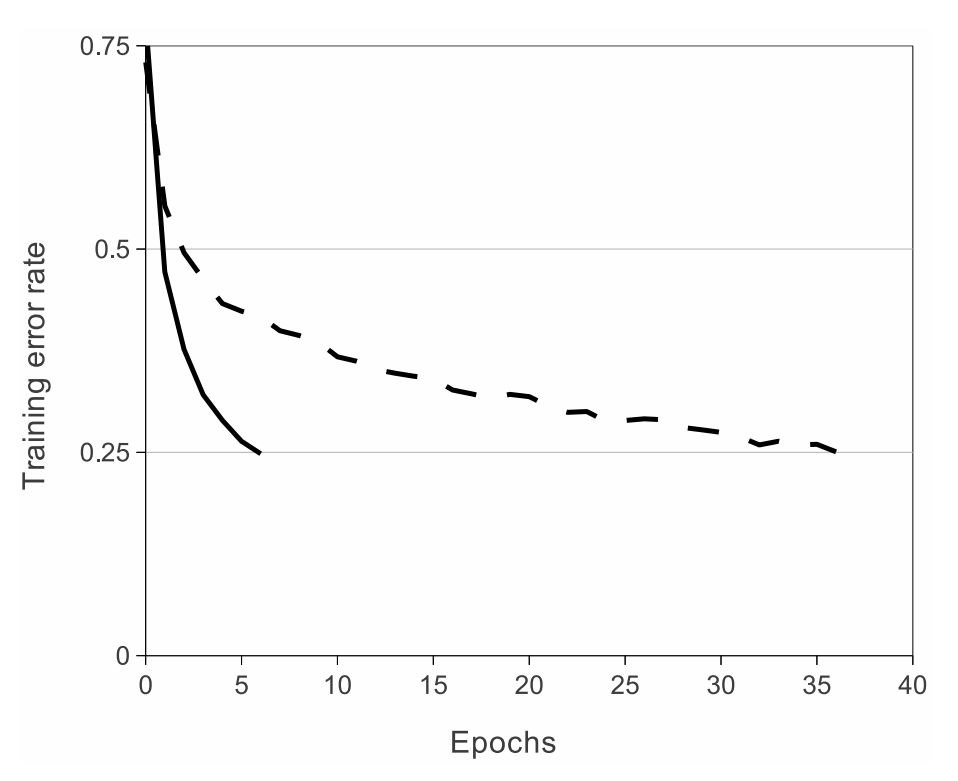
\includegraphics[width=0.7\linewidth]{img/01-01} \end{center}

Figure 1: A four-layer convolutional neural network with ReLUs \textbf{(solid line)} reaches a 25\% training error rate on CIFAR-10 six times faster than an equivalent network with tanh neurons \textbf{(dashed line)}. The learning rates for each network were chosen independently to make training as fast as possible. No regularization of any kind was employed. The magnitude of the effect demonstrated here varies with network architecture, but networks with ReLUs consistently learn several times faster than equivalents with saturating neurons.

\hypertarget{training-on-multiple-gpus}{%
\subsection{Training on Multiple GPUs}\label{training-on-multiple-gpus}}

A single GTX 580 GPU has only 3GB of memory, which limits the maximum size of the networks that can be trained on it. It turns out that 1.2 million training examples are enough to train networks which are too big to fit on one GPU. Therefore we spread the net across two GPUs. Current GPUs are particularly well-suited to cross-GPU parallelization, as they are able to read from and write to one another's memory directly, without going through host machine memory. The parallelization scheme that we employ essentially puts half of the kernels (or neurons) on each GPU, with one additional trick: the GPUs communicate only in certain layers. This means that, for example, the kernels of layer 3 take input from all kernel maps in layer 2. However, kernels in layer 4 take input only from those kernel maps in layer 3 which reside on the same GPU. Choosing the pattern of connectivity is a problem for cross-validation, but this allows us to precisely tune the amount of communication until it is an acceptable fraction of the amount of computation.

The resultant architecture is somewhat similar to that of the ``columnar'' CNN employed by Cire¸san et al.~{[}5{]}, except that our columns are not independent (see Figure 2). This scheme reduces our top-1 and top-5 error rates by 1.7\% and 1.2\%, respectively, as compared with a net with half as many kernels in each convolutional layer trained on one GPU. The two-GPU net takes slightly less time to train than the one-GPU \(net^2\).

\hypertarget{local-response-normalization}{%
\subsection{Local Response Normalization}\label{local-response-normalization}}

ReLUs have the desirable property that they do not require input normalization to prevent them from saturating. If at least some training examples produce a positive input to a ReLU, learning will happen in that neuron. However, we still find that the following local normalization scheme aids generalization. Denoting by \(a^i_{x,y}\) the activity of a neuron computed by applying kernel i at position \((x, y)\) and then applying the ReLU nonlinearity, the response-normalized activity \(b^i_{x,y}\) is given by the expression


\backmatter
% \printindex

\end{document}
